\chapter{Proposed Methodology}
\label{chap:methodology}

In our proposed methodology, we aim to leverage the strengths of both the UniCL framework and the Swin Transformer architecture to enhance the performance of our model. The methodology is structured into several key components, each addressing a specific aspect of the overall process. The following sections provide a detailed overview of each component, including the backbone architecture, CAM generation, pseudo label generation, segmentation prediction, and refinement.

\section{Overview}
\label{sec:overview}
In this section, we provide a high-level overview of the proposed methodology. The methodology is designed to address the challenges of weakly supervised semantic segmentation (WSSS) by leveraging the strengths of multi-modal learning frameworks like UniCL and advanced vision architectures such as the Swin Transformer. The key components of the methodology include:

\begin{figure}
    \centering
    \fbox{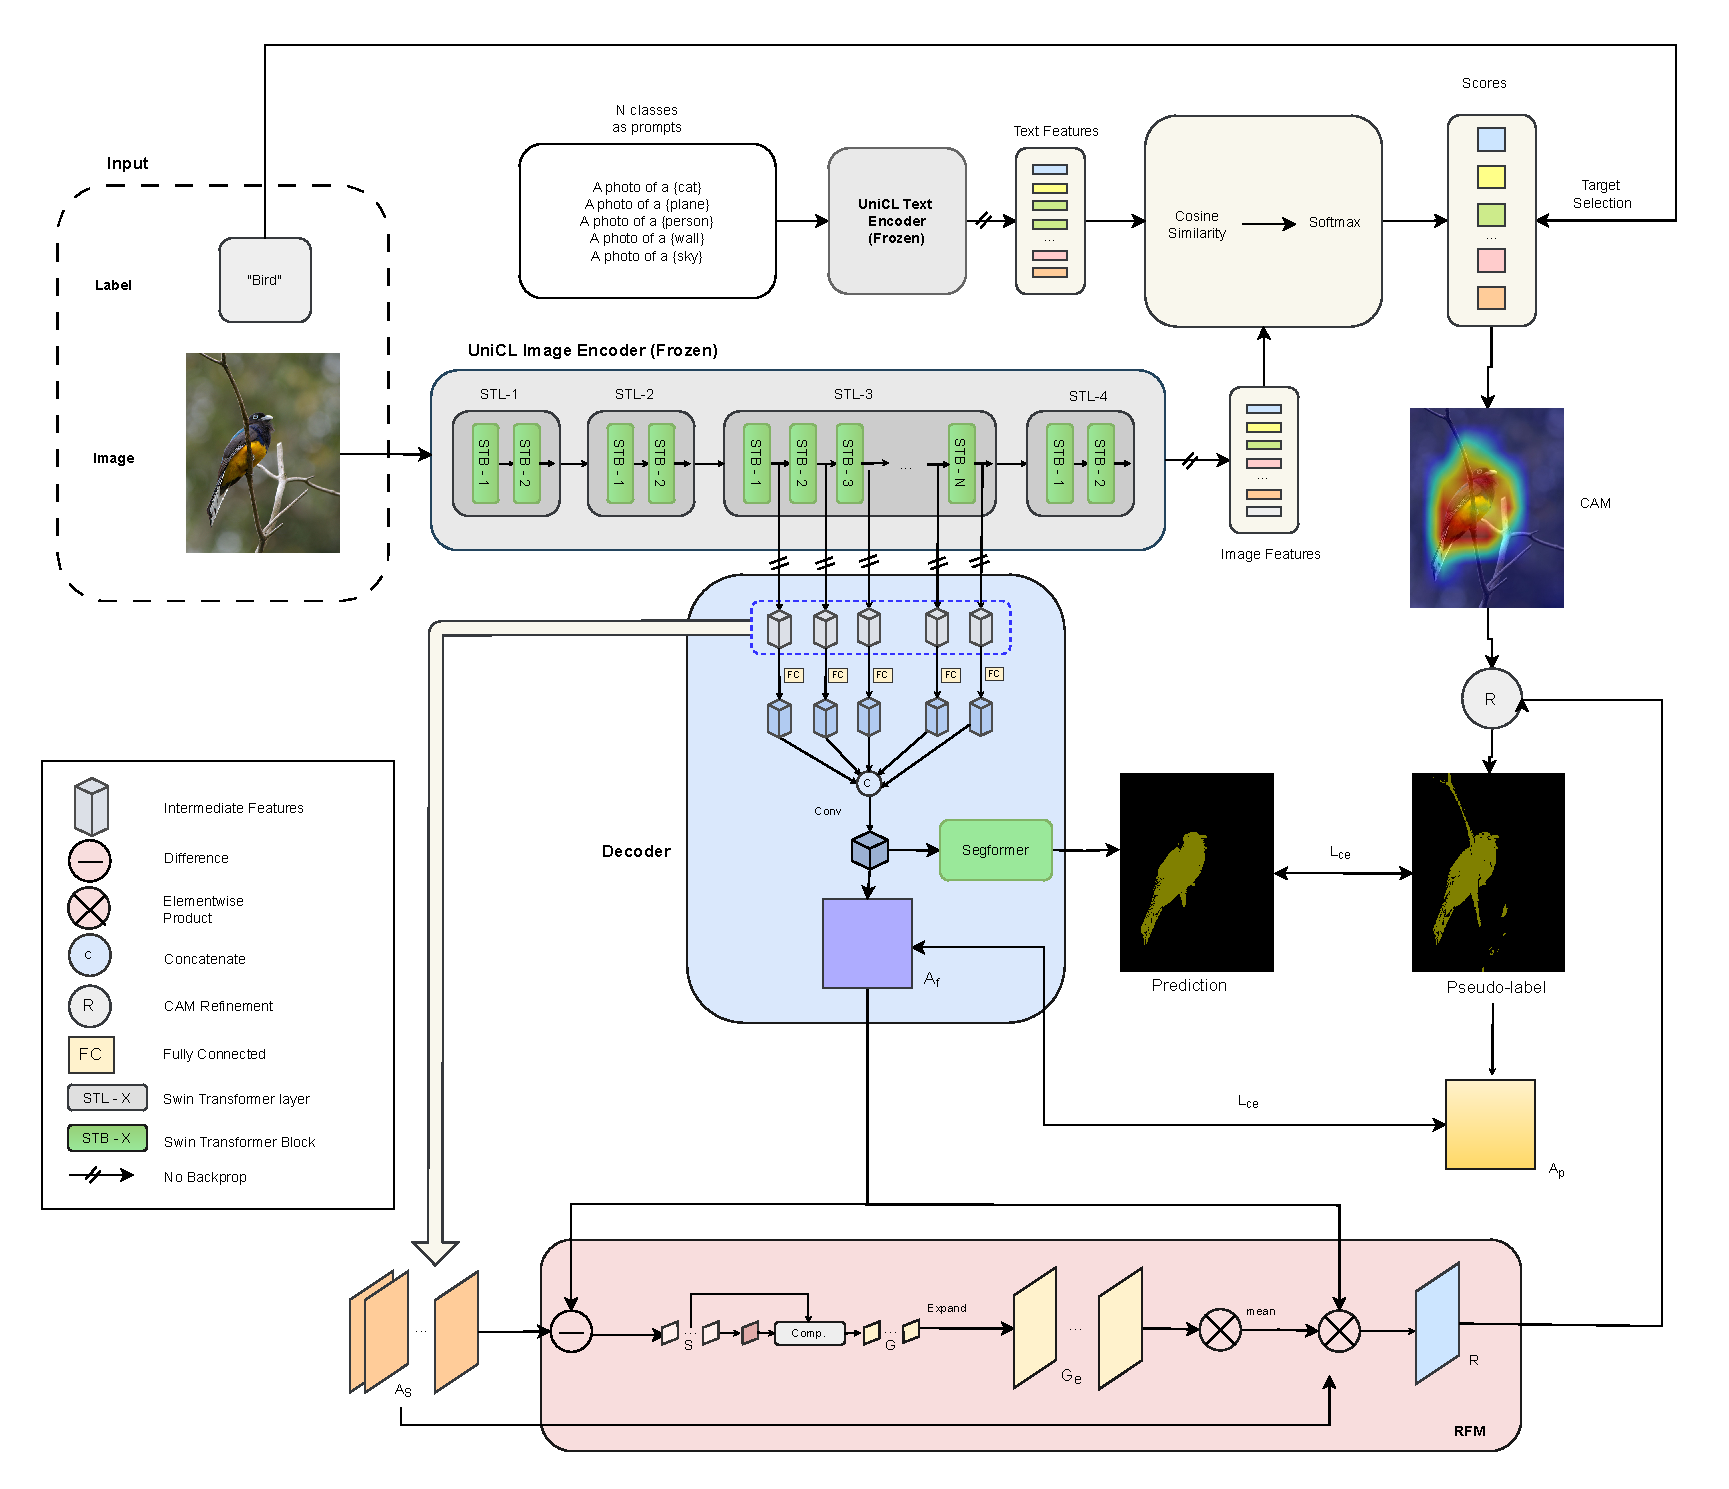
\includegraphics[width=0.98\textwidth, height = 1.05\textwidth]{figures/architecture}}
    \caption{Architecture of UniCL-AffSeg}
    \label{fig:architecture}
\end{figure}

\begin{itemize}
    \item \textbf{Feature Extraction from Backbone}: The backbone network is responsible for generating Class Activation Maps (CAMs) from input images. We experiment with UniCL as the backbone due to its multi-modal capabilities and state-of-the-art performance in generating high-quality CAMs.
    \item \textbf{CAM Generation}: CAMs are generated using Grad-CAM techniques adapted for multi-modal models like UniCL. These CAMs highlight the regions of interest in the image for each class.
    \item \textbf{Segmentation Prediction}: The feature maps from the backbone are aggregated and passed through a decoder to produce segmentation predictions. The decoder employs multi-head transformer layers to refine the predictions.
    \item \textbf{CAM Refinement and Pseudo-Label Generation}: Initial CAMs are refined using affinity-based techniques and random walk propagation to generate high-quality pseudo-labels. These pseudo-labels serve as supervision for training the segmentation model.
    \item \textbf{Loss Function}: A combination of segmentation loss and affinity loss is used to optimize the model. The affinity loss ensures consistency between the affinity maps of the decoder and the pseudo-labels, while the segmentation loss aligns the predictions with the refined CAMs.
\end{itemize}

The proposed methodology integrates these components into a cohesive framework, enabling the generation of accurate segmentation maps from weak supervision signals. \autoref{fig:architecture} illustrates the overall architecture of the proposed methodology, highlighting the flow of data through each component.


\section{Feature Extraction from Backbone}
\label{sec:feature_extraction_from_backbone}

In weakly supervised semantic segmentation (WSSS), two components play a crucial role: class activation maps (CAMs) and pseudo labels. The CAMs are first generated from the backbone network, and these are subsequently used to construct pseudo labels. The pseudo labels then serve as supervision for training the segmentation head—or the full segmentation model in the case of a multi-stage approach. 

The accuracy of the initial CAMs directly affects the quality of the pseudo labels and, consequently, the performance of the segmentation model. To achieve robust feature representations, we employ UniCL \cite{vl_unicl}, a multi-modal contrastive learning model built upon the CLIP framework. In this section, we first introduce CLIP, outlining its core architecture and characteristics. We then discuss UniCL and its innovations over CLIP, followed by a description of the Swin Transformer backbone that underpins the image encoding process.

\subsection{Contrastive Language-Image Pre-Training (CLIP)}
\label{subsec:clip}

CLIP \cite{vl_clip} is a multi-modal learning framework that utilizes contrastive learning to align images and text within a shared embedding space. It is designed to acquire representations that generalize well across different tasks without the need for task-specific fine-tuning. By training on extensive datasets of image-text pairs, CLIP learns to capture meaningful associations between visual and textual modalities.

\subsection{CLIP Architecture}
\label{subsec:clip_architecture}

\subsubsection{CLIP Components}
CLIP comprises two principal components:

\begin{itemize}
    \item \textbf{Image Encoder}: Responsible for processing images and extracting feature representations. This typically involves a Swin Transformer, pooling layers, and additional modules to capture spatial hierarchies and relationships within image data.
    \item \textbf{Text Encoder}: Processes textual data and converts it into a format suitable for comparison with image features. It generally includes transformer layers and attention mechanisms to capture semantic relationships within the text.
\end{itemize}

CLIP is trained using a contrastive loss function that aligns image and text features in a shared embedding space. This enables the model to learn representations applicable to a variety of tasks, such as image classification, object detection, and image segmentation. In the context of this work, CLIP's capabilities are leveraged for weakly supervised semantic segmentation, which relies solely on image-level classification.

\subsection{Characteristics of CLIP}
\subsubsection{Multi-Modal Learning}
\label{subsec:multi_modal_learning}
Multi-modal learning involves integrating information from different modalities, such as images and text, to enhance model performance. By combining complementary cues from multiple sources, models can develop a deeper and more comprehensive understanding of the data. For instance, in classification tasks, leveraging both visual and textual data enables the model to capture more nuanced semantic relationships. A key advantage of this approach is the potential for zero-shot learning, where the model can recognize and classify images from previously unseen categories. This is accomplished by aligning visual features with corresponding textual descriptions, allowing the model to generalize beyond the training set. Such capabilities are particularly valuable, as classification often underpins many downstream applications.

\subsubsection{Contrastive Learning}
\label{subsec:contrastive_learning}
Contrastive learning is a self-supervised approach focused on learning representations by distinguishing between positive and negative pairs. The objective is to bring representations of related inputs (such as an image and its corresponding textual description) closer in a shared embedding space, while pushing apart representations of unrelated inputs. This is typically achieved using a contrastive loss function, which minimizes the distance between positive pairs and maximizes it for negative pairs. Such a strategy enables models to acquire robust, discriminative, and generalizable feature representations.

\subsubsection{Training Strategy}
\label{subsec:training_strategy}
The training strategy for multi-modal learning generally integrates both supervised and self-supervised techniques. Models are trained on large-scale datasets containing paired samples from different modalities, facilitating the learning of meaningful representations through methods such as contrastive learning. Data augmentation is commonly applied to enhance the diversity and robustness of the learned features, thereby improving the model's generalization to unseen data.

\subsubsection{Task-Agnostic Learning}
\label{subsec:task_agnostic_learning}
Task-agnostic learning refers to the development of representations that are not specialized for a single task but are applicable across a range of downstream applications. This is accomplished by focusing on learning generalizable features through training on diverse datasets and leveraging multi-modal information. As a result, models can adapt their learned representations to various tasks, including image classification, object detection, and image segmentation. This adaptability makes task-agnostic learning a valuable approach for constructing versatile and reusable models.

\subsection{Unified Contrastive Learning (UniCL)}
\label{subsec:unicl}

UniCL, or Unified Contrastive Learning \cite{vl_unicl}, is a multi-modal learning framework that extends the ideas of CLIP by unifying different contrastive learning strategies within a single architecture. This enables more effective and flexible learning from multiple modalities.

UniCL is more than a straightforward extension of CLIP; it introduces several important innovations to improve both performance and adaptability.

A key feature of UniCL is its unified approach to contrastive learning, integrating image-label and text-label associations into a joint image-label-text space. This unified framework allows the model to leverage more positive pairs during training. While CLIP treats only the provided image-text pair as a positive match, UniCL recognizes that multiple text descriptions or images can correspond to the same category. For instance, both "a photo of a cat" and "a photo of a kitten" may be valid positive pairs for an image of a cat. UniCL's contrastive loss encourages the model to learn similarities across all features sharing the same category, resulting in a more comprehensive and robust shared representation space for images and text.

\subsubsection{Unified Image-Text-Label Contrast in UniCL}
\label{subsec:unified_image_text_label_contrast}

UniCL employs a bidirectional learning objective between image-text pairs:
\begin{equation} \label{eq:unified_image_text_label_contrast}
    \min_{\{\theta, \phi\}} \mathcal{L}_{\text{BiC}} = \mathcal{L}_{i2t} + \mathcal{L}_{t2i},
\end{equation}
where \(\mathcal{L}_{i2t}\) and \(\mathcal{L}_{t2i}\) are the image-to-text and text-to-image contrastive losses, respectively. And \(\theta\) and \(\phi\) are the parameters of the image and text encoders, respectively.

To align the representations of images and their corresponding textual descriptions within a batch, the image-to-text contrastive loss is formulated as follows. This loss encourages the model to associate each image with all relevant text features that share the same class label, thereby strengthening the alignment between visual and textual modalities in the shared embedding space:
\begin{equation} \label{eq:unicl_image_to_text_contrastive_loss}
    \mathcal{L}_{i2t} = - \sum_{i \in \mathcal{B}} \frac{1}{|\mathcal{P}(i)|} \sum_{k \in \mathcal{P}(i)} 
    \log \frac{\exp(\tau \mathbf{u}_i^\top \mathbf{v}_k)}{\sum_{j \in \mathcal{B}} \exp(\tau \mathbf{u}_i^\top \mathbf{v}_j)},
\end{equation}
where $k \in \mathcal{P}(i) = \{k | k \in \mathcal{B}, y_k = y_i\}$, i.e., the set of all images in the batch that belong to the same class as image $i$.

Conversely, the text-to-image contrastive loss, which aligns each text feature in a batch with its corresponding image features, is formulated as:

\begin{equation} \label{eq:unicl_text_to_image_contrastive_loss}
    \mathcal{L}_{t2i} = - \sum_{j \in \mathcal{B}} \frac{1}{|\mathcal{P}(j)|} \sum_{k \in \mathcal{P}(j)} 
    \log \frac{\exp(\tau \mathbf{u}_k^\top \mathbf{v}_j)}{\sum_{i \in \mathcal{B}} \exp(\tau \mathbf{u}_i^\top \mathbf{v}_j)},
\end{equation}
where $k \in \mathcal{P}(j) = \{k \mid k \in \mathcal{B}, y_k = y_j\}$, i.e., the set of all text features in the batch that belong to the same class as text $j$.

\subsubsection{Comparison with CLIP}
\label{subsec:clip_vs_unicl}

In case CLIP, for an image, there is only one positive text feature. In other words, $\mathcal{P}(i) = {i} \in \mathcal{B}$; and $\mathcal{P}(j) = {j} \in \mathcal{B}$. So, the image-to-text contrastive loss is defined as:

\begin{equation} \label{eq:clip_image_to_text_contrastive_loss}
    \mathcal{L}_{i2t} = - \sum_{i \in \mathcal{B}} 
    \log \frac{\exp(\tau \mathbf{u}_i^\top \mathbf{v}_i)}{\sum_{j \in \mathcal{B}} \exp(\tau \mathbf{u}_i^\top \mathbf{v}_j)},
\end{equation}
where $i \in \mathcal{B}$ is the index of the image in the batch.

And the text-to-image contrastive loss is defined as:

\begin{equation} \label{eq:clip_text_to_image_contrastive_loss}
    \mathcal{L}_{t2i} = - \sum_{j \in \mathcal{B}} 
    \log \frac{\exp(\tau \mathbf{u}_j^\top \mathbf{v}_j)}{\sum_{i \in \mathcal{B}} \exp(\tau \mathbf{u}_i^\top \mathbf{v}_j)},
\end{equation}
where $j \in \mathcal{B}$ is the index of the text feature in the batch. 

The equations \ref{eq:unified_image_text_label_contrast}-\ref{eq:clip_text_to_image_contrastive_loss} are taken from \cite{vl_unicl}.

This means that $\mathcal{L}_{BiC}$ becomes CLIP training objective. The main property in \autoref{eq:unicl_text_to_image_contrastive_loss} is that for each image feature, any of the text features in the batch can be used as a positive pair. And so is the case for \autoref{eq:unicl_text_to_image_contrastive_loss}.

Second, UniCL replaces CLIP's ViT backbone with a Swin Transformer backbone. The Swin Transformer is a hierarchical vision transformer that captures both local and global information in images, making it more suitable for various vision tasks.

\subsection{Swin Transformer}
\label{subsec:swin_transformer}
The Swin Transformer \cite{transformer_swin} is a hierarchical vision transformer architecture that utilizes a shifted windowing mechanism to effectively capture both local and global image information. It is engineered for computational efficiency while delivering strong performance across a range of computer vision tasks. The model is organized into multiple stages, each comprising distinct transformer blocks, which enables the processing of images at varying resolutions and facilitates the extraction of multi-scale features.

\autoref{fig:swin_vs_vit_architecture} presents a comparative overview of the Swin Transformer and Vision Transformer (ViT) architectures. The principal difference between the two lies in their respective processing paradigms: the Swin Transformer adopts a hierarchical framework, operating on feature maps at multiple scales, whereas ViT processes the entire image globally at a single resolution. This hierarchical design empowers the Swin Transformer to simultaneously capture fine-grained local details and broader contextual information, making it particularly advantageous for applications that demand both.

Within the Swin Transformer, hierarchical feature maps are constructed by progressively merging image patches (shown in gray) at deeper network layers. Self-attention is computed exclusively within localized windows (indicated in red), resulting in linear computational complexity with respect to the input image size. This approach not only enhances efficiency but also renders the Swin Transformer highly suitable for dense prediction tasks, such as image segmentation and classification.

Conversely, conventional vision transformers like ViT generate feature maps at a single, lower resolution and apply self-attention globally, which incurs quadratic computational complexity relative to the input size. While global attention can be beneficial for certain tasks, it is less efficient for dense recognition scenarios compared to the localized attention employed by the Swin Transformer.

\begin{figure}[htbp]
    \centering
    \fbox{ % Draw a box around the entire figure
        \begin{minipage}{0.9\textwidth} % Adjust the width as needed
            \begin{subfigure}[b]{0.45\textwidth}
                \centering
                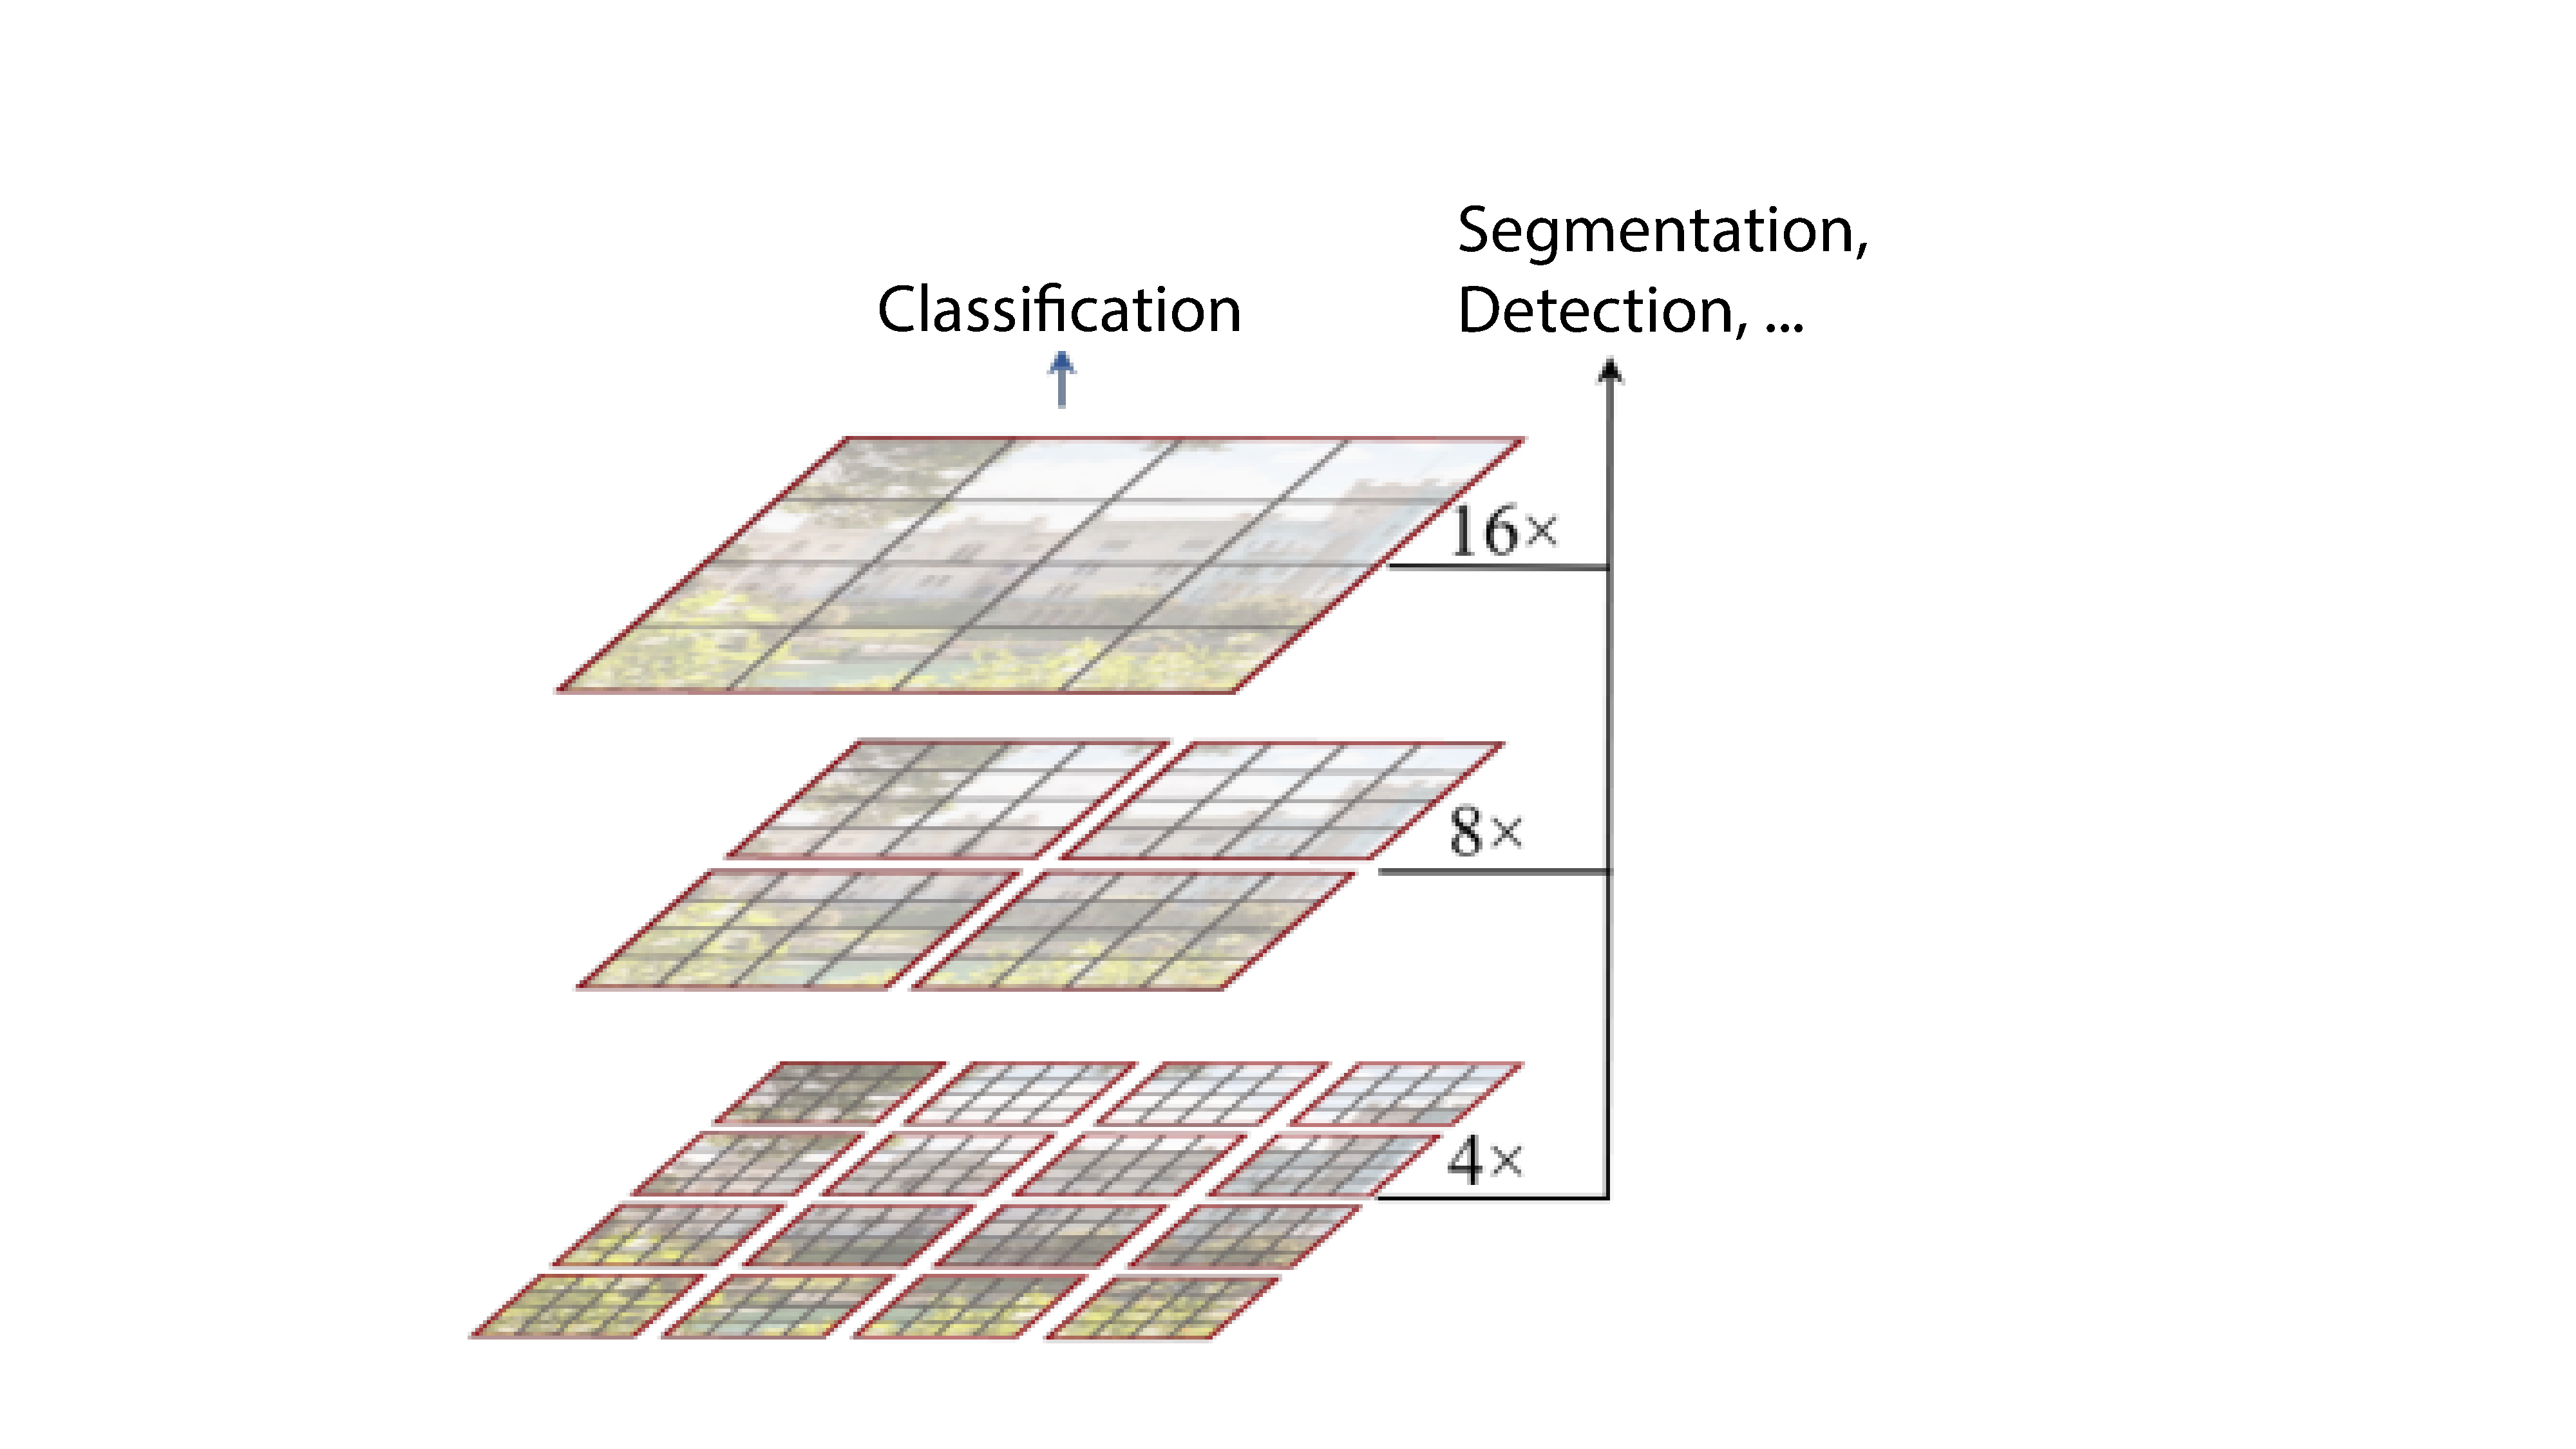
\includegraphics[width=\textwidth]{swin-vs-vit-archi-a.pdf}
                \caption{Swin Transformer}
                \label{fig:swin_transformer_data_flow}
            \end{subfigure}
            \hfill
            \begin{subfigure}[b]{0.45\textwidth}
                \centering
                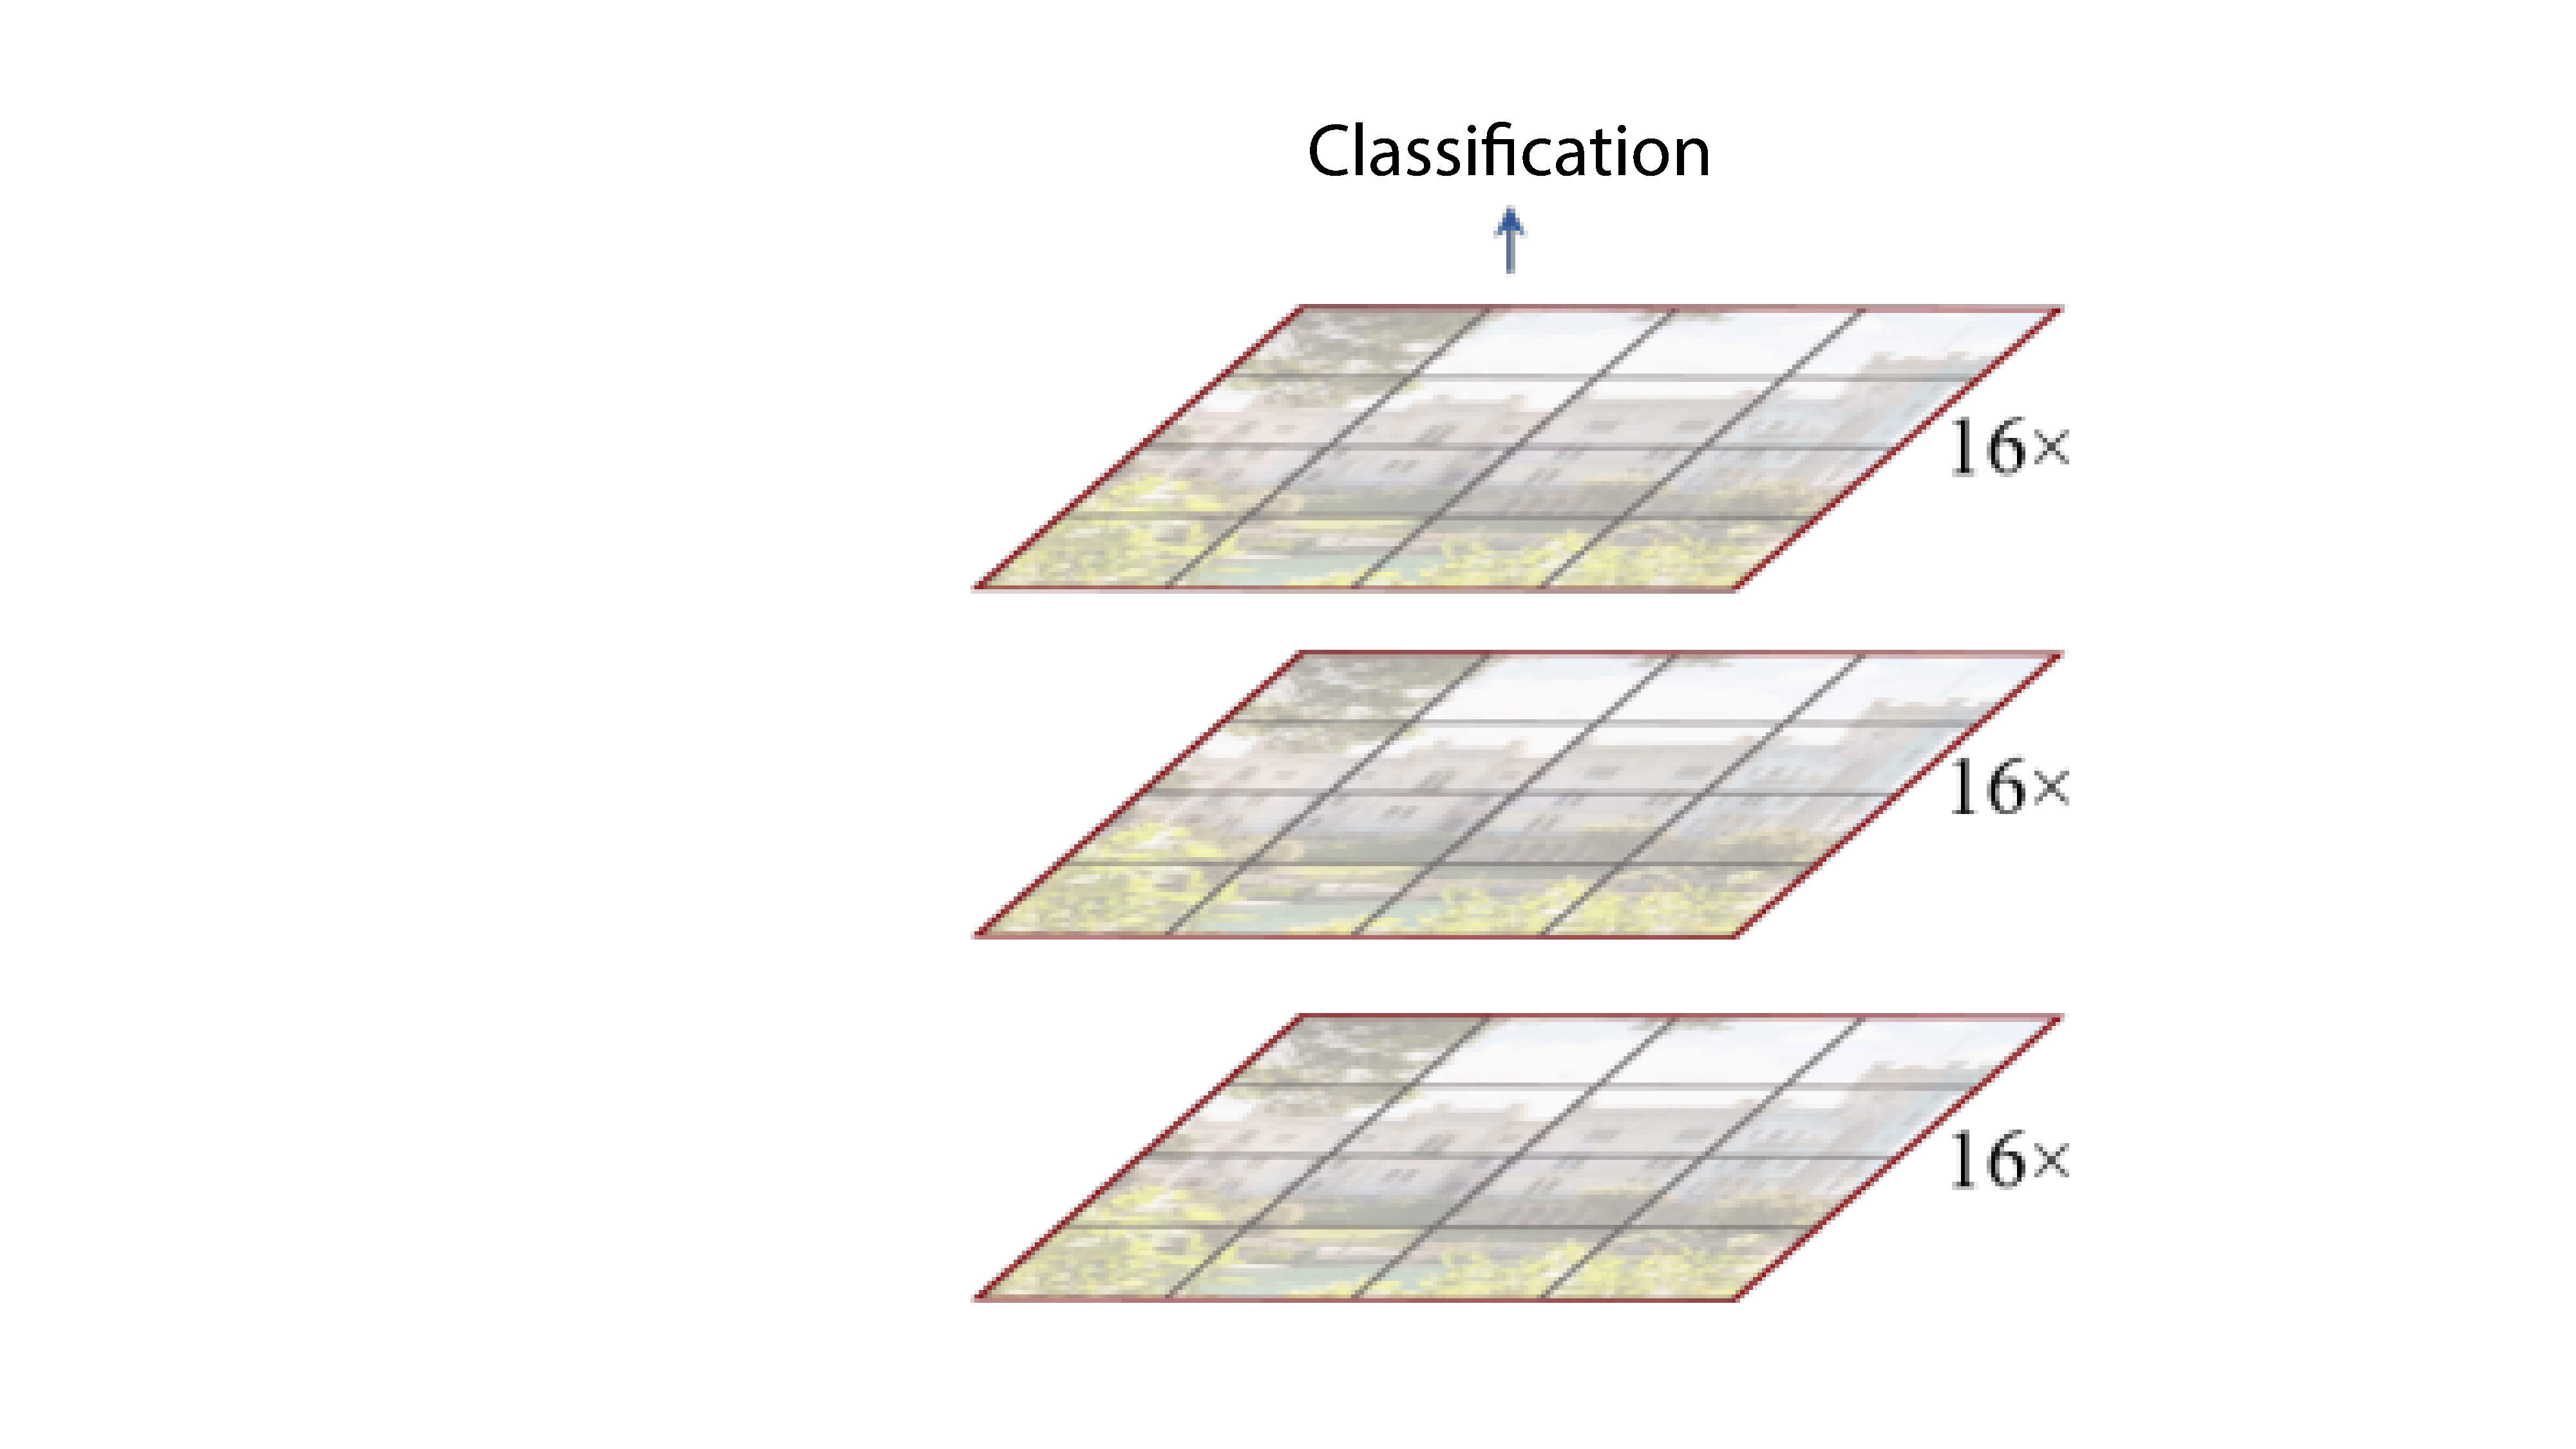
\includegraphics[width=\textwidth]{swin-vs-vit-archi-b.pdf}
                \caption{Vision Transformers}
                \label{fig:vit_data_flow}
            \end{subfigure}
        \end{minipage}
    }
    \caption{Comparison of Swin Transformer and ViT Architectures}
    \label{fig:swin_vs_vit_architecture}
\end{figure}

Owing to its hierarchical structure, the Swin Transformer is exceptionally well-suited for tasks that necessitate the integration of global context—essential for discerning the overall image structure—and local information, which is critical for identifying intricate features such as edges and textures. This makes it a compelling choice for image segmentation applications.

Furthermore, integrating the contrastive and multi-modal learning strengths of UniCL with the Swin Transformer’s hierarchical design can significantly enhance the model’s capacity to learn robust and discriminative representations from both visual and textual data. This synergy facilitates a more holistic understanding of multimodal inputs, thereby improving overall model performance.

With this foundational context established, the subsequent section details the proposed methodology, which comprises several core components: the backbone architecture, class activation map (CAM) generation, pseudo-label creation, segmentation prediction, and refinement. Each of these elements is integral to optimizing the model’s effectiveness.


\begin{figure}[ht]
  \centering
  \setlength{\tabcolsep}{2pt} % adjust spacing
  \renewcommand{\arraystretch}{0.9}
    \centering
    % CAMs with class labels on the left
    \begin{tabular}{c c} % first column = label

    % Column headers
    (a) Original Image & (b) CAM \\
    [1mm]
    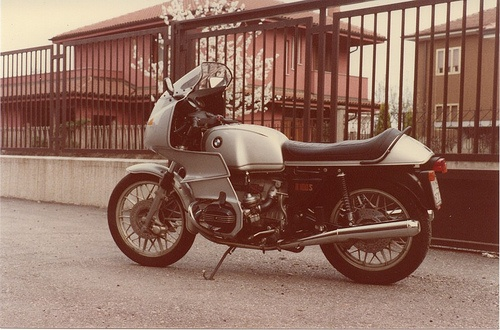
\includegraphics[width=0.3\textwidth,height=0.3\textwidth]{figures/originals/2007_002260}
    & 
    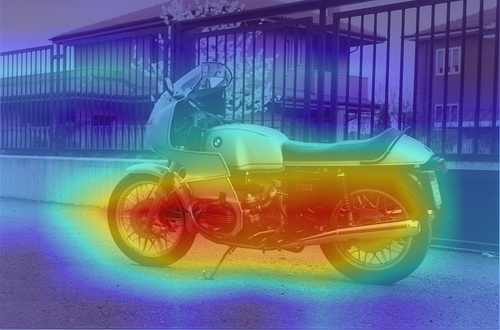
\includegraphics[width=0.3\textwidth,height=0.3\textwidth]{figures/test_cams/ours/2007_002260_13}
    \\
  \end{tabular}

  \caption{Original image and CAM generated by our method for class \textit{Motorbike}.}
  \label{fig:cam_examples}
\end{figure}

\section{CAM Generation}
\label{sec:cam_generation}

\autoref{fig:cam_generation_process_clip} shows the process of generating CAMs using CLIP/UniCL. We have used Grad-CAM. The process is similar to the method discussed in \autoref{subsec:grad_cam}, which is used to generate CAMs using CNN-based models.
 But there are some differences.

AS CLIP is a multi-modal model, the main classification task is to find similarity between the image and text. If we want to generate the CAM for $N$ classes, we need to provide $N$ text features as input. So, at the very beginning, we need to encode the text features using the CLIP text encoder, and store them.

An MLP layer takes the linear combination of the input features and the weights. We do the same thing when finding similarity score between the image and text features, take the linear combination of the image features and the text features. So, we can consider these text features as the "neuron weights" of the classifier head.

Then, we need to pass the image through the CLIP image encoder to get the feature maps. The rest of the process is the same as Grad-CAM. An example of the produced CAM for the \textit{Motorbike} class is shown in \autoref{fig:cam_examples}.


\begin{figure}[htbp]
    \centering
    \fbox{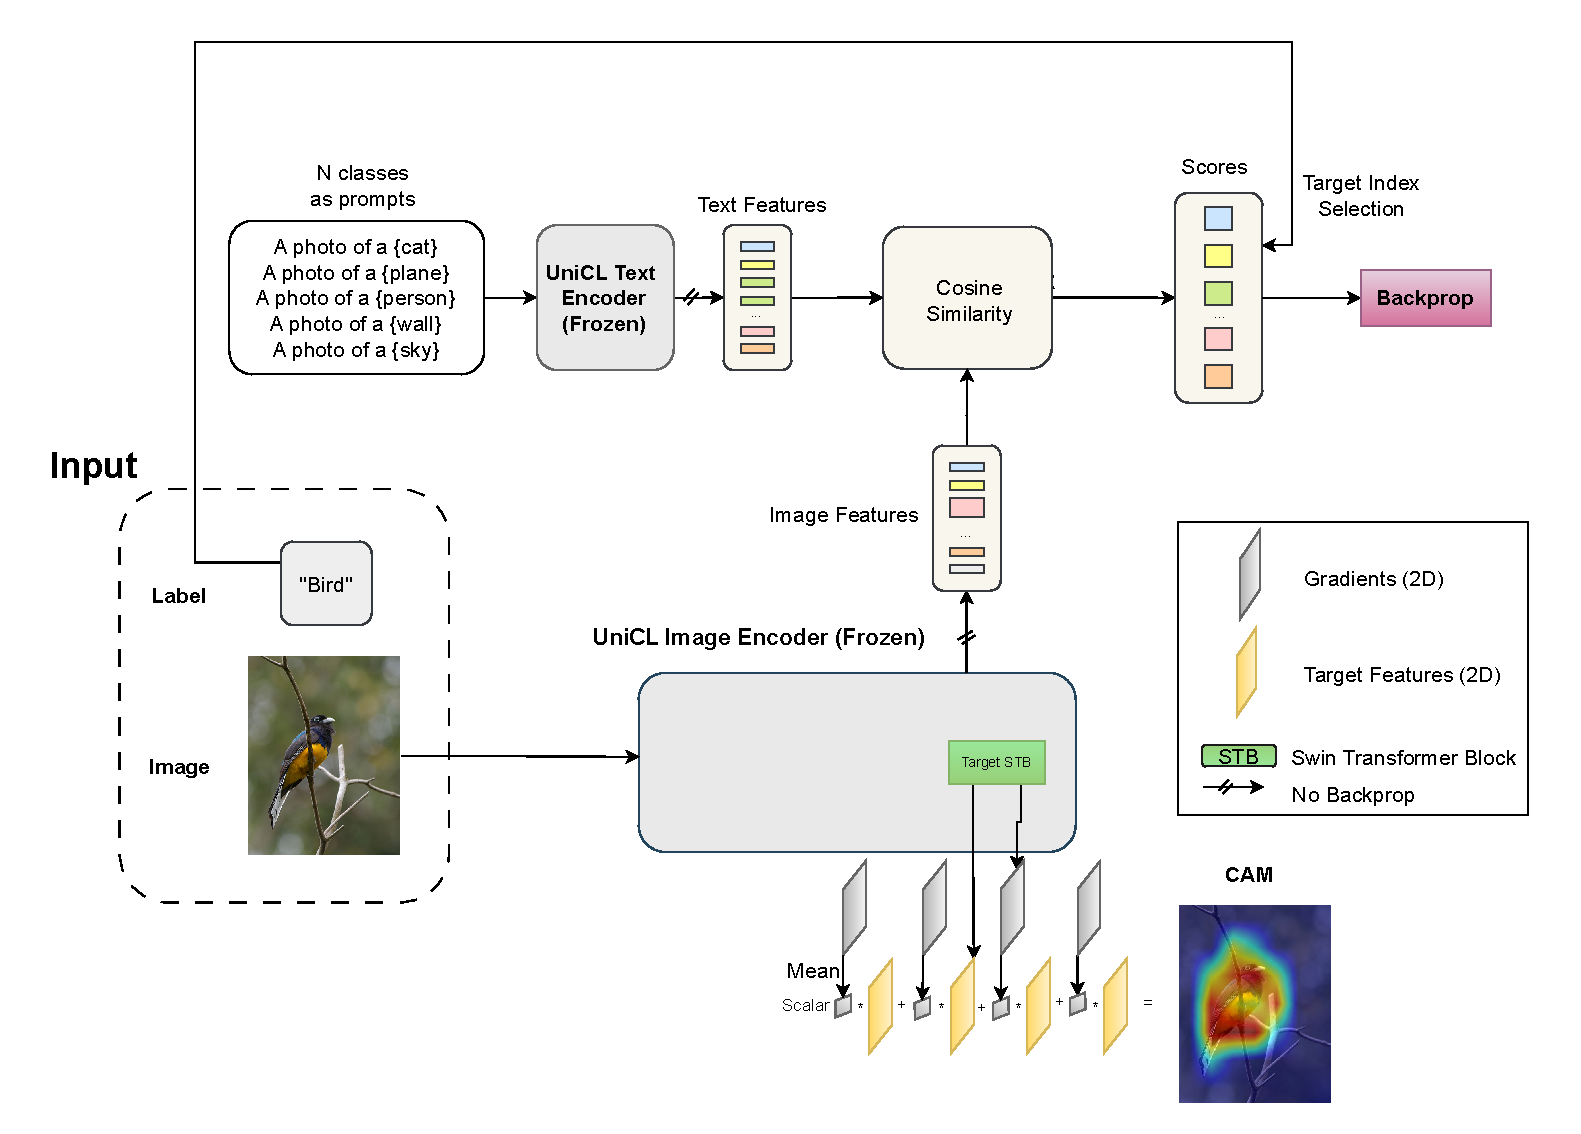
\includegraphics[width=0.8\textwidth]{methodology_cam.pdf}}
    \caption{CAM Generation Process using UniCL}
    \label{fig:cam_generation_process_clip}
\end{figure}

\section{Segmentation Prediction}
\label{sec:segmentation_prediction}
The segmentation prediction module is responsible for producing pixel-level class predictions for the input image. It comprises two primary stages: aggregation of encoder features and a decoder built with multi-head transformer layers. The design is inspired by the approach in \cite{wsss_frozen_clip}.

\subsection{Encoder Feature Aggregation}
\label{subsec:en_feature_agg}
In accordance with the methodology outlined in \cite{wsss_frozen_clip}, the feature representations extracted from each transformer block of the UniCL image encoder \cite{vl_unicl} are forwarded to the decoder for further processing. Denote the output feature map from the $l$-th transformer block as \( F_l^{\text{init}} \), where \( l = 1, \dots, N \). To harmonize the feature dimensions and enhance representational capacity, each \( F_l^{\text{init}} \) is individually transformed via a dedicated multilayer perceptron (MLP). Specifically, the transformation is defined as:
\begin{equation}
    F_l^{\text{new}} = W_{1}^{\text{fc}} \left( \text{ReLU} \left( W_{2}^{\text{fc}}(F_l^{\text{init}}) \right) \right),
\end{equation}
where \( W_{1}^{\text{fc}} \) and \( W_{2}^{\text{fc}} \) denote learnable fully connected layers, and \(\text{ReLU}(\cdot)\) represents the rectified linear unit activation function. This procedure ensures that the multi-scale features from different encoder stages are suitably projected for subsequent aggregation and decoding.


After that, all new feature maps \( F_l^{\text{new}} \) for \( l = 1, \dots, N \) are concatenated together, which are then processed by a convolution layer to generate a fused feature map \( F_u \):
\begin{equation}
    F_u = \text{Conv}\left( \text{Concat}\left[ F_1^{\text{new}}, F_2^{\text{new}}, \dots, F_N^{\text{new}} \right] \right),
    \tag{2}
\end{equation}

where \( F_u \in \mathbb{R}^{d \times h \times w} \), and \( d \), \( h \), and \( w \) represent the channel dimension, height, and width of the feature map, respectively. \(\text{Conv}(\cdot)\) is a convolutional layer, and \(\text{Concat}[\cdot]\) denotes the concatenation operation.


\subsection{Generating Final Prediction}
\label{subsec:decoder_final_pred}

Several sequential multi-head transformer layers are designed to generate the final prediction \( P \):
\begin{equation}
    \label{eq:prediction}
    P = \text{Conv}(\phi(F_u)) \uparrow,
\end{equation}
where \( P \in \mathbb{R}^{C \times H \times W} \), \( C \) is the number of classes including background, and \(\phi\) represents the sequential multi-head transformer blocks [12]. Each transformer block contains a multi-head self-attention module, a feed-forward network, and two normalization layers. The operator \(\uparrow\) denotes an upsampling operation to align the prediction map size with the original image.


\section{CAM Refinement and Pseudo-Label Generation}
\label{sec:refinement}
\subsection{Affinity based CAM refinement}  
The initial CAMs produced by the backbone tend to focus only on sparse, highly discriminative regions. These activations are often noisy and insufficient to be used directly as supervision. Therefore, a refinement module is required where the initial CAM is improved. The refined CAM is then used as a pseudolabel for supervision.  

The most common strategy for rectifying CAMs is by exploiting the feature relationships within the backbone that generates them. This is referred to as affinity-based CAM refinement, first introduced by \cite{wsss_affinitynet}. In transformer-based backbones, the attention maps naturally encode semantic-level affinities between tokens or patches. From these attention maps, an affinity matrix $A_f$ can be constructed and employed for CAM refinement via random walk propagation. In parallel, another affinity matrix, $A$, can be derived from the predicted pseudolabel produced by the decoder. The cross-entropy loss between these two affinity matrices is then incorporated into the training objective.  

However, in our case, the backbone responsible for generating the CAMs is \textbf{frozen}, meaning that its attention maps remain fixed and do not update during training. To address this limitation, Frozen CLIP \cite{wsss_frozen_clip} proposes utilizing the affinity derived from intermediate features of the encoder instead of directly relying on the backbone’s frozen attention. The backbone attention maps are then used only to influence this encoder-derived affinity, producing a final refined matrix $R$, which is further transformed into a transition matrix $T$ for random walk propagation.  

\begin{figure}[t]
    \centering
    \fbox{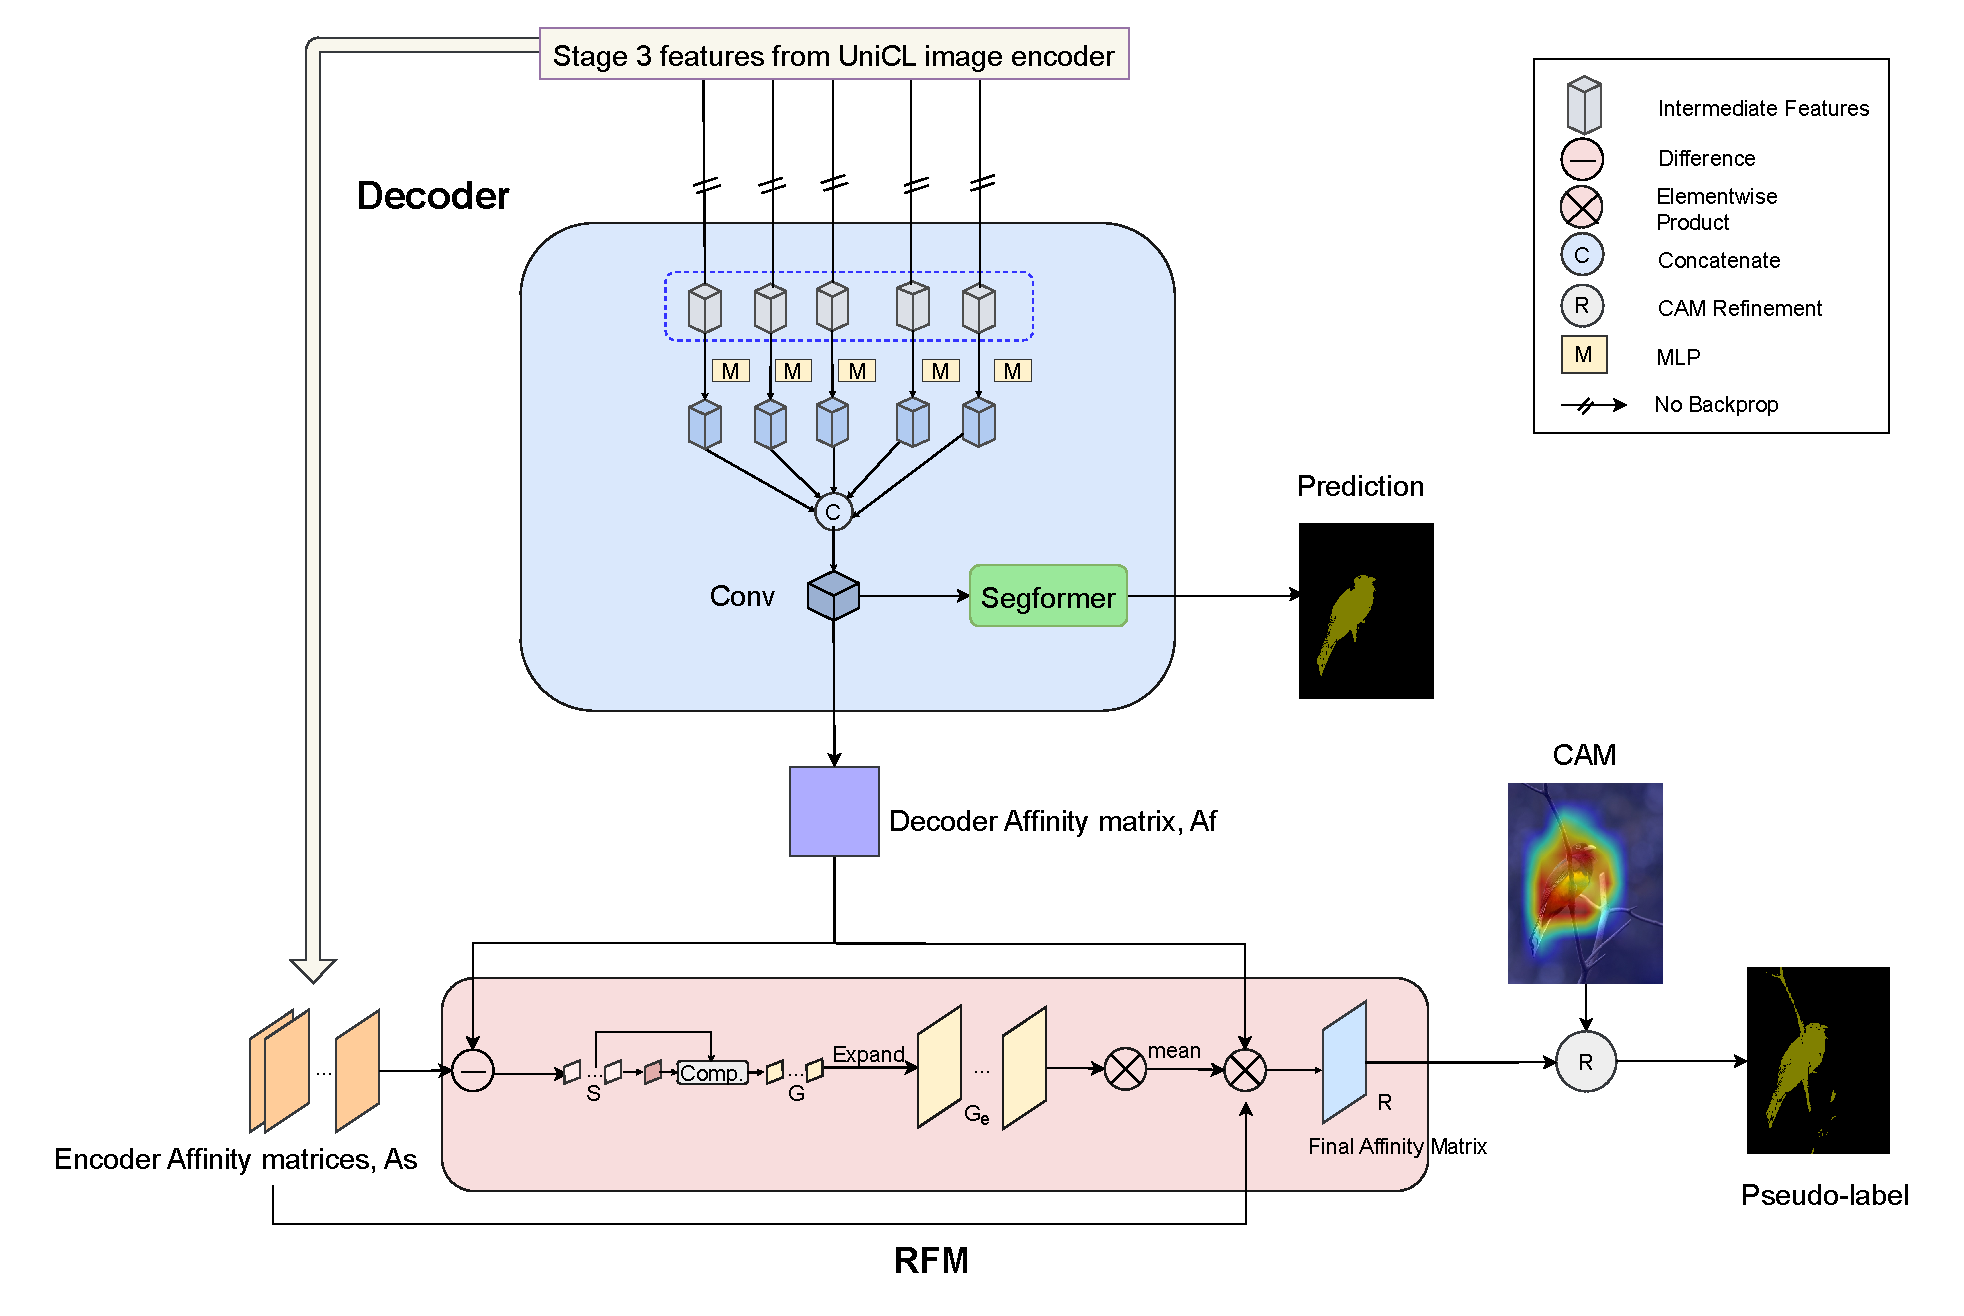
\includegraphics[width=0.9\textwidth]{figures/DecoderRFM}}
    \caption{Decoder and Refinement Module}
    \label{fig:decoder}
\end{figure}

In our setup, the UniCL backbone is based on the Swin Transformer, whose shifted-window design restricts the attention mechanism to \textbf{local regions}. Consequently, the attention maps fail to capture the \textbf{global semantic affinities} necessary for effective CAM propagation, and we could not use them directly for refinement. To overcome this, we compute affinities from the \textbf{intermediate feature maps of the Swin encoder}.  

Formally, let $f^{(k)} \in \mathbb{R}^{C \times L}$ denote the feature map from the $k$-th encoder block, where $C$ is the channel dimension and $L = h \times w$ represents the flattened spatial resolution. Each feature map is first normalized along the channel dimension:

\begin{equation}
\tilde{f}^{(k)}_i = \frac{f^{(k)}_i}{\| f^{(k)}_i \|_2}, \quad i = 1, \dots, L
\end{equation}

The affinity between spatial positions $i$ and $j$ within block $k$ is then computed as the dot-product similarity:

\begin{equation}
A^{(k)}_{ij} = \tilde{f}^{(k)}_i{}^\top \tilde{f}^{(k)}_j
\end{equation}

We compute such affinity matrices across multiple intermediate encoder blocks to capture complementary semantic relations at different abstraction levels. The resulting set of affinities is represented as:

\begin{equation}
\mathcal{A} = \{ A^{(1)}, A^{(2)}, \dots, A^{(N)} \}, \quad \mathcal{A} \in \mathbb{R}^{N \times hw \times hw}
\end{equation}

This multi-block affinity representation provides richer contextual cues for propagating and refining class activation maps.


\subsection{Extracting affinity map from the decoder}
\label{subsec:decoder_aff_mat}
Based on the feature map $F_u$ obtained from the decoder (as defined in Eq.~(2)), an affinity map is constructed as follows:

\begin{equation}
    \label{eq: A_f}
    A_f = \text{Sigmoid}(F_u^\top F_u),
\end{equation}

where $F_u \in \mathbb{R}^{d \times h \times w}$ is reshaped into a matrix of size $d \times hw$ before the computation. The $\text{Sigmoid}(\cdot)$ function ensures that the values in the resulting affinity map lie in the range $[0, 1]$. Consequently, the computed affinity map $A_f$ has the dimensions $\mathbb{R}^{hw \times hw}$. Here, $\top$ denotes the matrix transpose.

\subsection{Selecting affinity maps of the image encoder}
\label{subsec:att_map_encoder}
Following \cite{wsss_frozen_clip}, we extract all the affinity maps from the frozen CLIP image encoder, denoted as $\{A^l\}_{l=1}^N$, where each affinity map $A^l \in \mathbb{R}^{hw \times hw}$. To evaluate the reliability of each affinity map $A^l$, we compare it with the previously computed decoder affinity map $A_f$ using the following deviation score:

\begin{equation}
    S^l = \sum_{i=1}^{hw} \sum_{j=1}^{hw} \left| A_f(i, j) - A^l(i, j) \right|,
\end{equation}

where $S^l$ quantifies how much the affinity map (encoder) $A^l$ deviates from the reference affinity (decoder) $A_f$.  

Based on this score, we assign a binary weight $G^l$ to each affinity map:  

\begin{equation}
    G^l =
    \begin{cases}
        1, & \text{if } S^l < \dfrac{1}{N - N_0 + 1} \sum_{m=N_0}^N S^m, \\[8pt]
        0, & \text{otherwise}.
    \end{cases}
\end{equation}

Here, $G^l \in \{0,1\}$ is expanded to $G^l_e \in \mathbb{R}^{hw \times hw}$ for subsequent operations. The threshold is chosen as the average of the scores $\{S^m\}_{m=N_0}^N$ from the later layers of the encoder. If $S^l$ is lower than this threshold, the corresponding affinity map is considered reliable and retained ($G^l = 1$); otherwise, it is filtered out ($G^l = 0$).  

This selection mechanism ensures that only high-quality affinity maps consistent with the encoder-derived relationships are preserved, thereby improving the robustness of the CAM refinement process.  

\subsection{Utilizing the frozen encoder affinity maps}
\label{subsec: mul_attn_and_aff}
Using the affinity map $A_f$ and the filtered affinity maps of the encoder, we construct a refining map $R$ by weighing the decoder affinity matrix with the mean of the selected encoder affinity maps. This method of selection is adopted first by \cite{wsss_frozen_clip}. The equation is given as:

\begin{equation}
    R = A_f \odot \frac{ \sum_{l=1}^N G^l_e A^l}{N_m},
\end{equation}

where $\odot$ denotes element-wise multiplication, and $N_m$ is the number of valid encoder affinity maps that have passed the filtering stage, defined as:

\begin{equation}
    N_m = \sum_{l = N_0}^N G^l.
\end{equation}

Here, $G^l_e \in \mathbb{R}^{hw \times hw}$ is the expanded binary filter corresponding to $G^l$. The refining map $R$ effectively integrates the reliable encoder affinity maps weighted by the affinity map $A_f$, enhancing meaningful relationships while suppressing noisy or irrelevant information.

\subsection{Constructing the semantic transition matrix}
\label{subsec:trans_mat}
Now that we have the affinity matrix $R$, to apply the random walk propagation, we need to at first normalize the rows for converting it into a transition probability matrix. In addition, column normalization ensures consistency and symmetric behavior. Sinkhorn normalization \cite{math_sinkhorn} is thus used to convert $R$ into a double stochastic matrix $R_{\text{nor}}$.

Next, $R_{\text{nor}}$ is converted into a symmetric matrix by adding its transpose and normalizing the sum:

\[
    T = \frac{R_{\text{nor}} + R_{\text{nor}}^T}{2}, \quad \text{where} \quad R_{\text{nor}} = \text{Sinkhorn}(R)
\]

The matrix $T$ is now symmetric whose rows and columns are normalized. This is the transition probability matrix to be used for random walk.


\begin{figure}[tbp]
    \centering
    \fbox{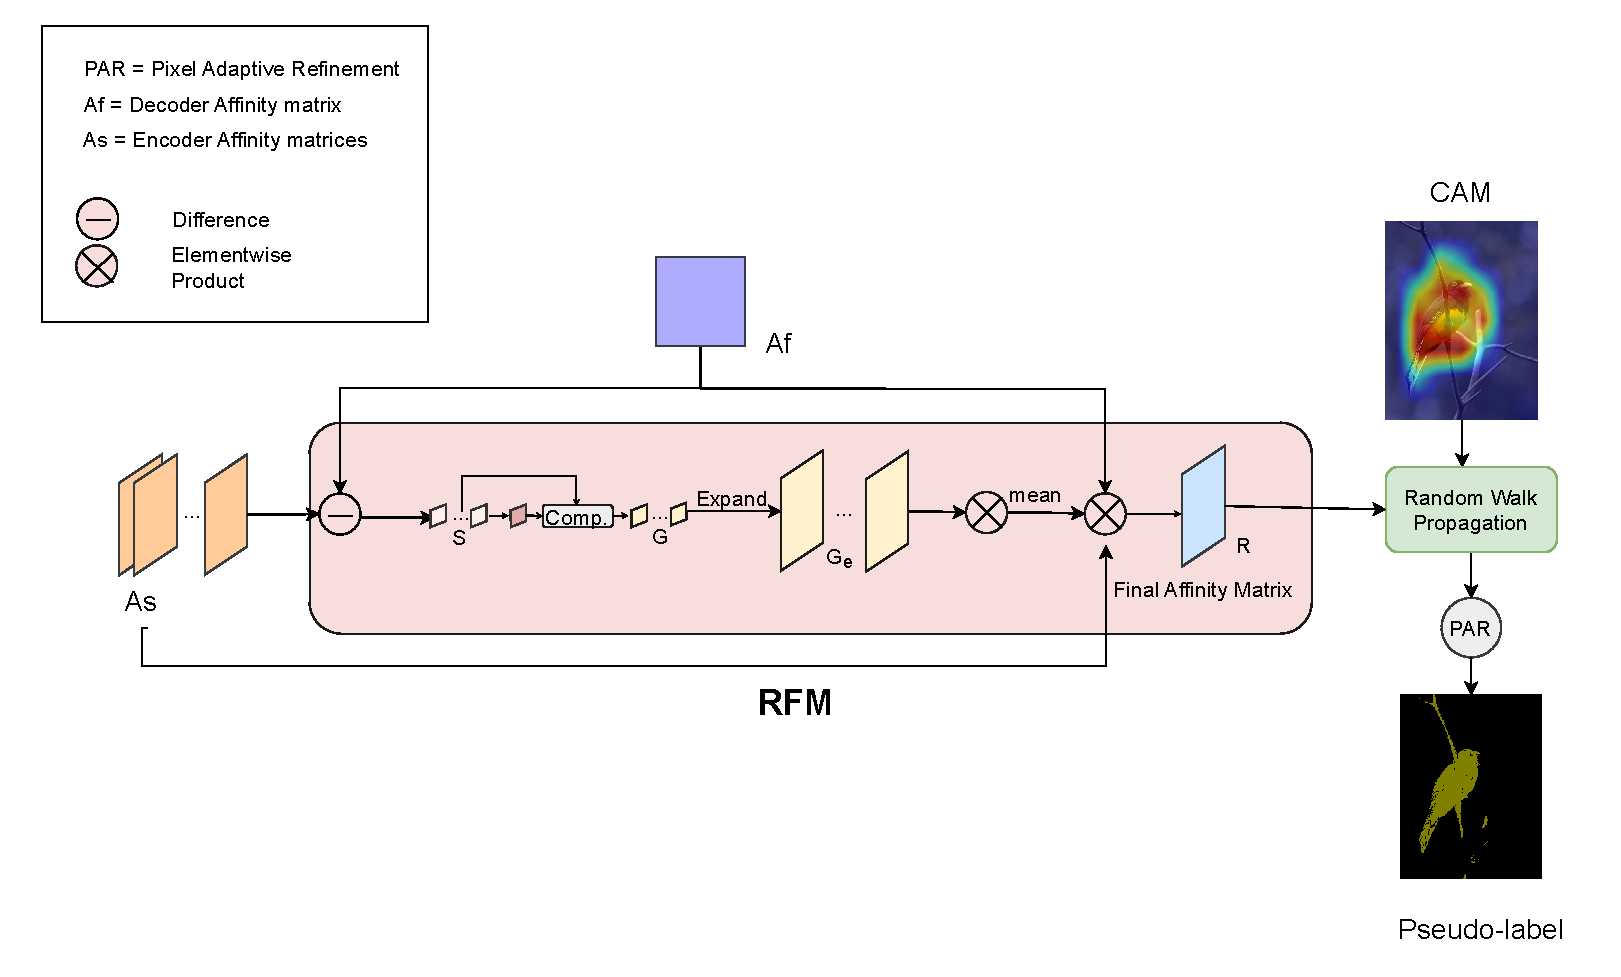
\includegraphics[width=0.95\textwidth]{figures/RFM}}
    \caption{CAM refinement by exploiting affinity map}
    \label{fig:refinement}
\end{figure}

\subsection{Random Walk Propagation}
\label{subsec:random_walk}

The refined class activation map (CAM) for a specific class $c$, denoted as $M^c_f$ is found by random walk propagation as follows:

\begin{equation}
    M_f^c = B^c \odot T^\alpha \cdot M_{\text{init}}^c
\end{equation}

where, $M^c_{\text{init}} \in \mathbb{R}^{hw \times 1}$ is the initial CAM for class $c$, reshaped into vector form. $T$ is the transition probability matrix, $\alpha$ is the hyperparameter that controls the strength of the refinement we want to apply. It is equivalent to the number of iterations of the random walk propagation. \( B^c \in \mathbb{R}^{1 \times hw} \) is the box mask obtained from the CAM of class \( c \), and \( \odot \) denotes the Hadamard product. This masking is needed to restrict the refining region spatially. It is obtained for each target class c by thresholding the CAM of this class by a constant. The connected regions of the mask map are found and covered by minimum rectangle bounding boxes. These boxes mask the affinity of distant pixels, preventing over-expansion.

Finally, the refined CAM $M^c_f$ is passed through an online post-processing module - specifically, the pixel-adaptive refinement module proposed in \cite{wsss_afa_affinity_from_attention}.

\subsection{Pixel Adaptive refinement module}
\label{subsec:par}
To ensure local consistency, pixel-adaptive convolution is introduced by \cite{wsss_afa_affinity_from_attention}. It uses local RGB and spatial information to define the low-level pair-wise semantic affinity of two pixels. Given an input image \( I \in \mathbb{R}^{h \times w \times 3} \), the pairwise affinities between two pixels at positions \((i, j)\) and \((k, l)\) is calculated as follows:

- \( \kappa^{\text{rgb}}_{ij,kl} \) measures color similarity (the closer the colors, the higher the affinity).

- \( \kappa^{\text{pos}}_{ij,kl} \) measures spatial closeness (pixels closer in space have higher affinity).

These are defined as:

\[
    \kappa^{\text{rgb}}_{ij,kl} = -\frac{\| I_{ij} - I_{kl} \|^2}{w_1 \sigma^2_{\text{rgb}}}, \quad
    \kappa^{\text{pos}}_{ij,kl} = -\frac{\| P_{ij} - P_{kl} \|^2}{w_2 \sigma^2_{\text{pos}}}
\]

Here:
- \( I_{ij} \) and \( P_{ij} \) are the RGB values and 2D spatial coordinates at pixel \((i, j)\),
- \( \sigma_{\text{rgb}} \) and \( \sigma_{\text{pos}} \) are the standard deviations of color and position differences,
- \( w_1 \) and \( w_2 \) are weights that control smoothness.

Then, the affinity kernel \( \kappa_{ij,kl} \) for each pixel pair is computed by applying a softmax to normalize both terms across the local neighborhood \( \mathcal{N}(i, j) \), and combining them:

\[
    \kappa_{ij,kl} = \frac{ \exp(\kappa^{\text{rgb}}_{ij,kl}) }{ \sum\limits_{(x, y) \in \mathcal{N}(i, j)} \exp(\kappa^{\text{rgb}}_{ij,xy}) }
    + w_3 \cdot \frac{ \exp(\kappa^{\text{pos}}_{ij,kl}) }{ \sum\limits_{(x, y) \in \mathcal{N}(i, j)} \exp(\kappa^{\text{pos}}_{ij,xy}) }
\]

Here, \( w_3 \) is a weight to balance the influence of the position term.

This affinity kernel is used to iteratively refine a CAM \( M \in \mathbb{R}^{h \times w \times C} \). At iteration \( t \), each pixel value \( M^t_{i,j,c} \) for class \( c \) is updated by aggregating class scores from neighboring pixels weighted by the affinity:

\begin{equation}
    M^t_{i,j,c} = \sum_{(k, l) \in \mathcal{N}(i, j)} \kappa_{ij,kl} \cdot M^{t-1}_{k,l,c}
\end{equation}


The neighborhood \( \mathcal{N}(i, j) \) is defined as the 8-connected neighbors (i.e., a \(3\times{3}\) window) with multiple dilation rates  allowing the refinement to capture both local and semi-local context.

\subsection{Pseudo-Label Generation}
\label{subsec:pseudo_label_generation}
The refined CAMs are used to generate the pseudo-labels or segmentation labels, which assign a class label to each pixel (patch),
\begin{equation}
    M_p(x, y) = \arg\max_{c \in \{1, \ldots, C\}} M_c(x, y)
\end{equation}
where \( M_c \in \mathbb{R}^{h \times w} \) is the refined CAM and \( M_p \in \mathbb{R}^{h \times w} \) is the pseudo-label.
The generated pseudo-labels are used as supervision for the segmentation network.



\section{Loss Function}
\label{subsec:loss_func}

The loss function defined by \cite{wsss_frozen_clip}:
\begin{equation}
    \mathcal{L} = \mathcal{L}_{seg} + \lambda \mathcal{L}_{aff}
\end{equation}

where, $\mathcal{L}_{aff}$ is the affinity loss and $\mathcal{L}_{seg}$ is the segmentation loss. $\lambda$ is the weighting parameter.
\subsection{Affinity Loss}
\label{aff_loss}

In the refinement module, we used the affinity map of the decoder features, $A_f$ (\autoref{eq: A_f}). The quality of the final pseudolabel directly depends on it. We need to ensure that the pairwise affinity of the pseudolabel matches the pairwise affinity of the decoder output, because that is what the random walk propagation implies.
We compute the affinity labels for the predicted pseudolabel as follows:

\begin{equation}
    A_p = O_h(M_p)^TO_h(M_p)
\end{equation}
where $O_h(.)$ is the one-hot encoding of $M_p$, and $A \in \mathbb{R}^{hw \times hw}$  is the affinity label.
. This means that the value of $A_p(i,j)$ will be 1 for the $(i,j)$ pair which have the same class label, and 0 otherwise. The affinity loss is the Cross-Entropy Loss of $A_f$ and $A_p$:
\begin{equation}
    \mathcal{L}_{aff} = \mathcal{L}_{ce}(A_f, A_p)
\end{equation}

\subsection{Segmentation Loss}
\label{seg_loss}
We obtain the segmentation prediction, $P$, from the decoder (\autoref{eq:prediction}). As we are using the refined CAM or pseudolabel, $M_p$ as supervision, the segmentation loss is computed:

\begin{equation}
    \mathcal{L}_{seg} = \mathcal{L}_{ce}(P, M_p \uparrow)
\end{equation}

where \( L_{ce} \) is the cross-entropy loss, and \( M_p{\uparrow} \in \mathbb{R}^{H \times W} \). $H$ and $W$ are the original height and width of the image respectively.


